\documentclass{beamer}
\usepackage{graphicx} % Required for inserting images
\usetheme{Madrid}
\usepackage{tikz}

%Customising my arrows 
\tikzstyle{box} = [rectangle, rounded corners, minimum width=3cm, minimum height=1cm,text centered, draw=black, fill=blue!10]
\tikzstyle{arrow} = [thick,->,>=stealth]

\title{Housing Supply and Elasticities}
\author{Abigail Meloche \& Tie Ma}
\date{February 25, 2025}

\begin{document}
\maketitle

\begin{frame}
\frametitle{Research Question \& Motivation}
\vspace{-1.5cm}
\begin{block}
{Question} Do higher housing supply elasticities cause housing supply and, consequently, housing prices to respond more strongly to monetary policy changes?
\end{block}
\bigskip{}

\textbf{Motivation}
\begin{itemize}
    \item Strong precedence for analyzing housing supply using elasticities in the literature
    \item Lack of empirical work on monetary policy and housing supply
\end{itemize}
\end{frame}

\begin{frame}
\frametitle{Motivation in Theory}
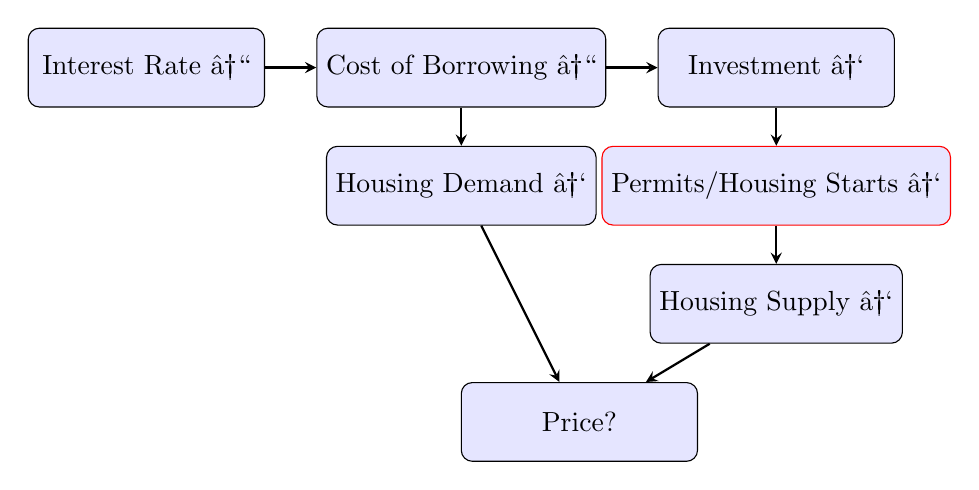
\begin{tikzpicture}[node distance=1cm]

\node (rate) [box] {Interest Rate ↓};
\node (borrowing) [box, right of= rate, xshift = 3cm] {Cost of Borrowing ↓};
\node (costs) [box, right of=rate, xshift=7cm] {Investment ↑};
\node (demand) [box, below of=borrowing, yshift=-0.5cm] {Housing Demand ↑};
\node (permits) [box, below of = costs, yshift = -0.5cm, draw = red] {Permits/Housing Starts ↑};
\node (supply) [box, below of = permits, yshift = -0.5cm] {Housing Supply ↑};
\node (price) [box, xshift = 5.5cm, yshift = -4.5cm] {Price?};

% Arrows
\draw [arrow] (rate) -- (borrowing);
\draw [arrow] (borrowing) -- (costs);
\draw [arrow] (borrowing) -- (demand);
\draw [arrow] (costs) -- (permits);
\draw [arrow] (permits) --(supply);
\draw [arrow] (supply) -- (price);
\draw [arrow] (demand) -- (price);

\end{tikzpicture}
\end{frame}



\begin{frame}
\frametitle{Motivation - Through The Data}
\begin{figure}
    \centering
    \includegraphics[width=0.9\linewidth]{Latex_Supply_Lagged_V2.png}
    \caption{12-Month Lagged Housing Supply \& Interest Rate}
    \label{fig:enter-label}
\end{figure}
\end{frame}



%%GET TO THIS
\begin{frame}
\frametitle{Data Availability}
\begin{itemize}
   \setlength{\itemsep}{1.5\baselineskip} % Adjust the spacing between items
    \item Statistics Canada Data
    \item 26 Census Metropolitan Areas (CMA's)
    \item Years: 1992-01-01 - 2019-12-01 
\end{itemize}
\end{frame}

\begin{frame}
\frametitle{Method - Step 1}
Compute housing elasticities using a log-log regression:
\medskip{}

\[
log(HousingSupply_{ij}) = \beta_1 *log(HousePrice_{ij}) + \epsilon_{ij}
\]
\smallskip{}

With i = city, j = year.
\end{frame}

\begin{frame}
\frametitle{Preliminary Results}
\begin{figure}
    \centering
    \includegraphics[width=0.9\linewidth]{Latex_elasticity.png}
    \caption{Relationship Between Housing Supply Elasticity \& Population Density (Left) and Logged Population (Right)}
    \label{fig:enter-label}
\end{figure}
\end{frame}



\begin{frame}
\frametitle{Method - Step 2}
\begin{itemize}
    \item Structural Vector Auto Regression (SVAR) model \& Cholesky Decomposition
    
\end{itemize}

%%ADD THE MATRIX
\[
A_0 =
\begin{bmatrix}
1 & 0 & 0 & 0 & 0 \\
a_{21} & 1 & 0 & 0 &0\\
a_{31} & a_{32} & 1 & 0 &0\\
a_{41} & a_{42} & a_{43} & 1 &0 \\a_{51} & a_{52} & a_{53} & a_{54} & 1
\end{bmatrix}
\]

\begin{enumerate}
    \item Construction costs
    \item Building permits
    \item Housing supply
    \item House prices
    \item Policy rate

%Construction costs respond first to external economic shocks (inflation, material price shifts, supply chain disruptions).
%Permits are granted next, as developers adjust investment plans based on costs and future expectations.
%Housing starts follow, given a lag between permits and actual construction.
%House prices adjust last, responding to supply-demand pressures.
%Interest rates are last, meaning monetary policy is influenced by changes in construction costs, building permits, housing supply and prices that occur in the same period. However, it doesn't impact the other variables contemporaneously 
\end{enumerate}
\end{frame}

\begin{frame}
\frametitle{Conclusion/Future Steps}
   
\begin{itemize}
\setlength{\itemsep}{1.5\baselineskip} % Adjust the spacing between items
    \item Consider control and/or instrumental variables in the elasticity regression
    \item Consider time series methods for elasticity calculations
    \item Determine appropriate lag length for SVAR 
\end{itemize}
\end{frame}

\begin{frame}

\centering
    \vspace{1.5cm}
    
    {\LARGE \textbf{Thank You!}} \\
    \vspace{0.6cm}
    
    {\Large Questions?} \\
    \vspace{1cm}
\end{frame}



%%%%%%%%%%%%%%%%%%
%Appendix Results%
%%%%%%%%%%%%%%%%%%

\begin{frame}
\frametitle{Appendix 1 - Regression Results}
\begin{table}[ht]
\centering
\begin{tabular}{l r l r}
  \hline
  CMA & Elasticity & CMA & Elasticity \\ 
  \hline
  Canada & 2.19 & Guelph & 0.69 \\ 
  St. John's & 0.88 & London & 1.30 \\ 
  Halifax & 1.08 & Windsor & 0.96 \\ 
  Quebec & 1.35 & Sudbury & 0.59 \\ 
  Sherbrooke & 0.99 & Winnipeg & 1.31 \\ 
  Trois Rivières & 0.82 & Regina & 1.09 \\ 
  Montreal & 1.71 & Saskatoon & 1.17 \\ 
  Ottawa-Gatineau & 1.43 & Calgary & 1.60 \\ 
  Oshawa & 0.58 & Edmonton & 1.63 \\ 
  Toronto & 1.65 & Kelowna & 1.14 \\ 
  Hamilton & 1.18 & Vancouver & 1.68 \\ 
  St. Catharines-Niagara & 1.08 & Victoria & 1.13 \\ 
  Kitchener-Waterloo & 1.18 & & \\ 
  \hline
\end{tabular}
\caption{Housing Supply Elasticities by CMA} 
\label{tab:elasticity}
\end{table}

\end{frame}

\begin{frame}
\frametitle{Appendix 2 - Average Housing Supply Rate of Change}
\begin{figure}
    \centering
    \includegraphics[width=1\linewidth]{Latex_ROC.png}
    \label{fig:enter-label}
\end{figure}
\end{frame}

